\documentclass{mathos}

\begin{document}
\renewcommand\bibname{Literatura}

\sloppy

\begin{titlepage}
\begin{center}
    
\includegraphics[keepaspectratio=true,scale=0.4]{MathosLogo.png} \\ \vspace{1mm}
       \textsc{Sveučilište Josipa Jurja Strossmayera u Osijeku} \\
    \vspace{2mm}
    \textsc{Fakultet primijenjene matematike i informatike}
\end{center}

\vspace{25mm}
\begin{center}
    % naslov
    {\LARGE{\bf  Kriptografija eliptičkih krivulja }}
    
    \vspace{15mm}
    %
    {\large{\sc Seminarski rad iz kolegija}}
    \break
    {\large{\sc suvremene teme iz računalne znanosti}}

\end{center}

\vspace{50mm}

\hfill
\begin{minipage}[t]{0.47\textwidth}\raggedleft
	{{Student:}{\normalsize\vspace{3mm} \bf\\ \large{Marin Kovač}}}
\end{minipage}

\vspace*{\fill}
\centering{\normalsize{Osijek, 2025.}}
\end{titlepage}


\chapter{Uvod}
\pagenumbering{arabic}

\bigskip
\noindent
Kriptografija eliptičkih krivulja (ECC\footnote{Elliptic-curve cryptography} u nastavku) jedan je od najmoćnijih kriptosustava javnog ključa. Bazirana je na svojstvima algebarske strukture eliptičkih krivulja nad konačnim poljima. Neovisno su je uveli Victor Miller i Neal Koblitz sredinom 1980-ih, ali se počela široko primjenjivati tek oko 2004. godine. ECC i njena primjena proizašla je iz potrebe za zadovoljavanjem zahtjeva moderne kriptografije. Primarna motivacija leži u postizanju superiornih razina sigurnosti u odnosu na tradicionalne kriptosustave poput RSA. To se prevodi u povećanu otpornost na napade grubom silom, te u novije vrijeme otpornost na kvantne napade. Uz to, važno je i poboljšanje učinkovitosti. ECC koristi manje veličine ključeva što rezultira bržim operacijama šifriranja/dešifriranja pa je posebno pogodan u okruženjima s ograničenim resursima (npr. čipovi).

Iako se o eliptičkim krivuljama i prostoru u kojem žive može pisati u beskraj, proći ćemo samo kroz osnovne definicije i ključne teoreme za razumjevanje principa na kojima je ECC zasnovan. Rad je pisan pod pretpostavkom da čitatelji imaju podlogu u kibernetičkoj sigurnosti, odnosno nemaju duboku matematičku podlogu o pojmovima vezanim za eliptičke krivulje te će se na što jednostavnij, ali svejedno formalan način, pokušati definirati i iskazati sve tvrdnje koje prethode metodi.


\chapter{Eliptičke krivulje}

\section{Uvodni pojmovi}
Kako bi uopče mogli definirati eliptičke krivulje, moramo poznavati neka svojstva elemenata nad kojima je ona definirana. Prisjetimo se u nastavku nekih osnovnih matematičkih pojmova.

\subsection{Grupa i polje}
\begin{defin}[Grupa]
    Skup $\mathbb{G}$ opremljen s binarnom operacijom ($\cdot:\mathbb{G}\times\mathbb{G} \to \mathbb{G}$) je \textbf{grupa} ako zadovoljava sljedeća svojstva:
    \begin{enumerate}
        \item Asocijativnost: $\\
            \forall a, b, c \in \mathbb{G}, \enspace a \cdot (b \cdot c) = (a \cdot b) \cdot c
            $
        \item Postojanje neutralnog elementa: $\\
            \exists e \in \mathbb{G} \enspace \text{takav da} \enspace \forall a \in \mathbb{G}, \enspace a \cdot e = e \cdot a = a
        $
        \item Postojanje inverznog elementa: $\\
            \forall a \in \mathbb{G}, \enspace \exists b \in \mathbb{G} \enspace \text{takav da} \enspace a \cdot b = b \cdot a = e, \enspace \text{gdje je e neutralni element}
        $
    \end{enumerate}
    Grupa $\mathbb{G}=(\mathbb{G}, \cdot)$ je \textbf{Abelova grupa} ako dodatno vrijedi:
    \begin{enumerate}
        \item Komutativnost: $\\
            \forall a, b \in \mathbb{G}, \enspace a \cdot b = b \cdot a
            $
    \end{enumerate}
\end{defin}

\begin{defin}[Polje]
    Skup $\mathbb{F}$ opremljen s dvije binarne operacije, zbrajanje ($+$) i množenje ($\cdot$), zovemo polje ako zadovoljava sljedeća svojstva:
    \begin{enumerate}
        \item $(\mathbb{F}, +)$ je Abelova grupa
        \item $(\mathbb{F}\setminus\{0\}, \cdot)$ je Abelova grupa
        \item Distributivnost množenja s obzirom na zbrajanje: $\\
            \forall a, b, c \in \mathbb{F}, \enspace a \cdot (b + c) = (a \cdot b) + (a \cdot c)
        $
    \end{enumerate}
\end{defin}

Lako se vidi da su skupovi $\mathbb{R}, \mathbb{Q}, \mathbb{Z}$ s uobičajenim operacijama zbrajanja i množenja polja. Navedeni primjeri polja su beskonačna polja, dok će nama od važnosti biti polja s konačnim brojem elemenata.

\begin{defin}[Karakteristika polja]
    Karakteristika polja (char($\mathbb{F}$)) je najmanji broj $n$ takav da
    \[ \underbrace{1 + \cdots + 1}_{n \text{ pribrojnika}} = 0 \]
    gdje su $1$ i $0$ redom neutralni element za množenje i neutralni element za zbrajanje.
    Ako takav $n$ ne postoji, onda $\text{char}(\mathbb{F}) = 0$.
\end{defin}

\subsection{Polinom}
\begin{defin}[Polinom]
    \textbf{Polinom} stupnja $n$ nad poljem $K$ je izraz oblika
    \[ a_nx^n + a_{n-1}x^{n-1} + ... + a_1x + a_0 \]
    gdje $a_i \in K$.
\end{defin}
\begin{defin}[Nultočka polinoma]
    Za $k \in K$ kažemo da je \textbf{korijen} ili \textbf{nultočka} polinoma $f(x)$ ako $f(k) = 0$.
\end{defin}
\begin{nap}
    Ako je $k$ nultočka, tada je $f(x)$ djeljiv polinomom $x - k$. Ako je $f(x)$ djeljiv polinomom $(x - k)^m$, ali nije djeljiv polinomom $(x - k)^{m+1}$, onda kažemo da je nultočka $k$ višestruka nultočka kratnosti $m$.
\end{nap}
\begin{defin}[Diskriminanta polinoma]
    Neka je $f(x)$ polinom stupnja $n$ i nultočkama $r_1, ..., r_n$.
    \textbf{Diskriminanta} $D$ polinoma $f(x)$ je
    \[ D = \prod_{i \neq j}^{} (r_i - r_j)^2 \]
\end{defin}
\begin{theorem}
    \label{th:dt}
    Determinanta polinoma jednaka je $0$ ako i samo ako $f(x)$ ima višestrukih nultočki.
\end{theorem}

\subsection{Projektivna ravnina}
Za definiciju eliptičke krivulje potrebno nam je poznavanje i prostora, odnosno ravnine u kojem krivulja živi. Eliptička krivulja je projektivna što znači da živi u projektivnoj ravnini.

Projektivnu ravninu možemo dobiti proširenjem afine\footnote{(Euklidska ravnina je vrsta afine ravnine)} ravnine ako napravimo sljedeće;
\begin{enumerate}
    \item Za svaki skup paralelnih pravaca proglasimo novu točku u kojoj se oni sijeku i nazovemo ju točka u beskonačnosti ($\mathcal{O}$)
    \item Za skup točaka u beskonačnosti proglasimo novi pravac koji nazivamo pravac u beskonačnosti i prolazi svim točkama u beskonačnosti
\end{enumerate}
Važno je primjetiti da se u projektivnoj ravnini, za razliku od afine, bilo koja dva pravca sjeku u točno jednoj točki.

Postoje razne međusobno ekvivalentne formalne definicije projektivne ravnine. Kako će naši iskazi i dokazi većinom biti elementarni, za projektivnu ravninu dat ćemo algebarsku definiciju.

\begin{defin}[Projektivna ravnina]
    Projektivna ravnina $\mathbb{P}^2(K)$ je kvocijentni skup\footnote{skup klasa ekvivalencije} od $K^3\setminus\{(0, 0, 0)\}$ po relaciji $\sim$. ($x \sim kx, \forall k \in K$)
\end{defin}
\begin{nap}
    Projektivnu ravninu nad K ćemo označavati s $KP^2$
\end{nap}

Iz definicije i ranije opisanog proširenja slijedi da se afina ravnina $K^2$ ugrađuje u projektivnu ravninu $KP^2$ preko preslikavanja afinih koordinata u homogene:
\[ (x, y) \mapsto (x, y, 1) \]
Komplement slike ovog preslikavanja su sve točke oblika $(x, y, 0)$. Upravo te točke su ranije definirane točke $\mathcal{O}$ koje zajedno definiraju pravac u beskonačnosti ($\{k(1, 0, 0) + m(0, 1, 0): k,m\in K\}$) u $K^3$.

\begin{primjer}
    Uzmimo neka dva pravca nagiba 0 u beskonačnoj afinoj ravnini. Možemo naslutiti da će se oni u projektivnoj ravnini sjeći u $(0, 1, 0)$. Neka su
    \[ u = \{(x, 0): x \in K\} \]
    \[ v = \{(x, 1): x \in K\} \]
    pravci u afinoj ravnini $K^2$ ($0$ i $1$ neutralni elementi pa su u $K$).
    Preslikavanjem u homogene koordinate dobijamo podskupe od $KP^2$;
    \[ \overset{\_}{u} = \{(x, 0, 1): x \in K\} \]
    \[ \overset{\_}{v} = \{(x, 1, 1): x \in K\} \]
    Da bi se u projektivnoj ravnini ovi podskupovi smatrali pravcima, moraju sadržavati točku u beskonačnosti u kojoj se sjeku s ostalim pravcima istog nagiba. Kako je točka projektivne ravnine klasa ekvivalencije omjera koordinata, kretanjem po x u beskonačnost konstante postaju beznačajno male s obzirom na x pa točku (0, 1, 0) prozivamo točkom u beskonačnosti. To znači da su skupovi $\overset{\_}{u} \cup \{(0, 1, 0)\}$ i $\overset{\_}{v} \cup \{(0, 1, 0)\}$ pravci u $KP^2$ i sjeku se u točki $\mathcal{O} = (0, 1, 0)$.
\end{primjer}

\begin{figure}[H]
    \begin{minipage}[c]{0.5\linewidth}
        \centering
        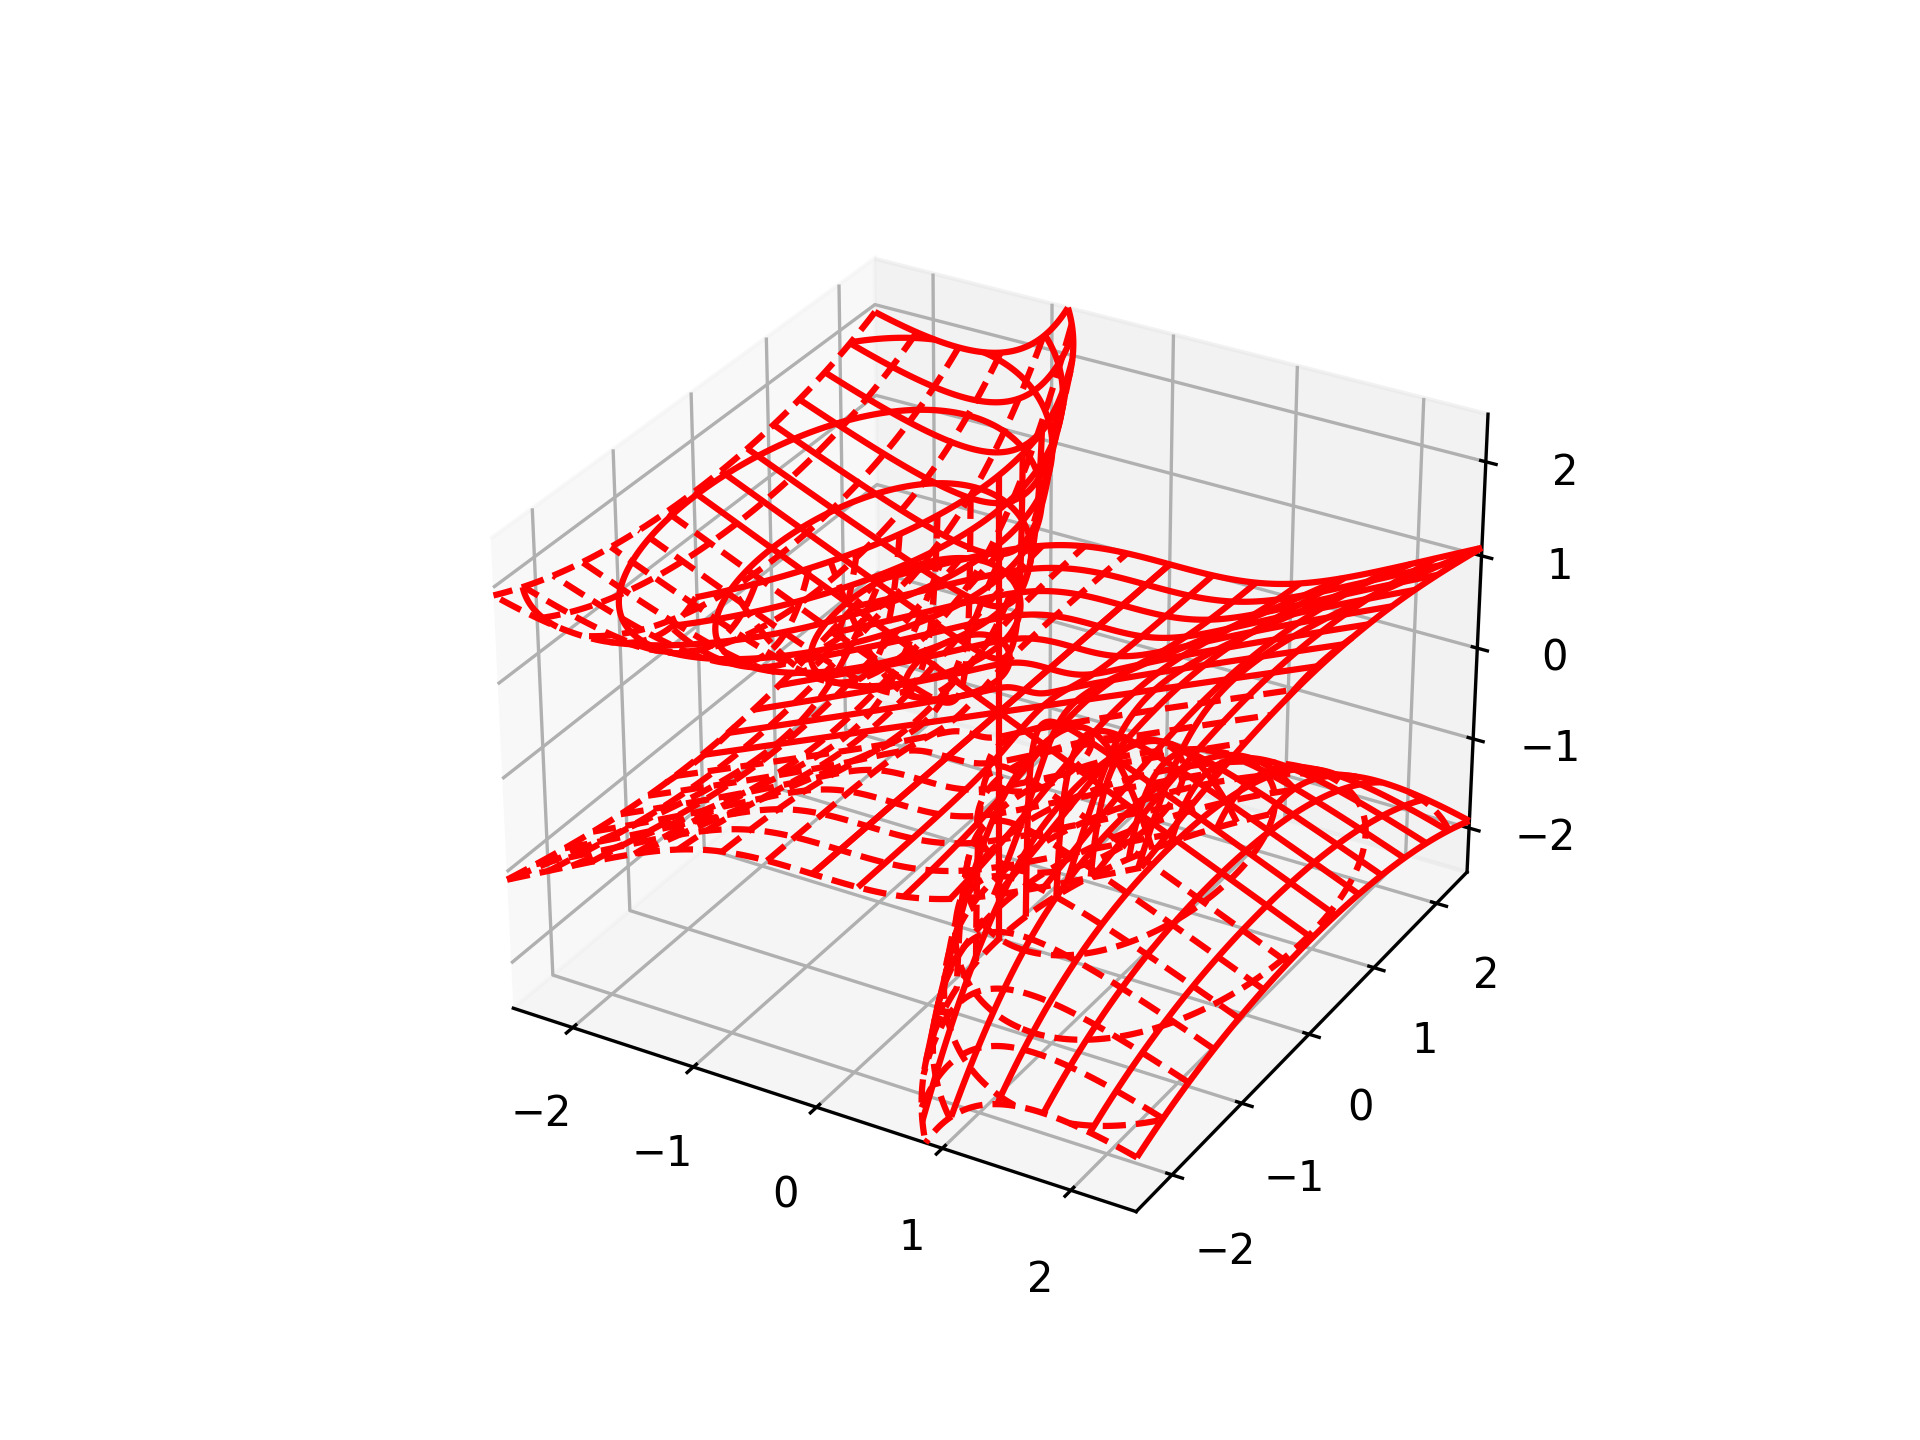
\includegraphics[width=\linewidth,keepaspectratio]{3.png}
    \end{minipage}
    \begin{minipage}[c]{0.4\linewidth}
        \centering
        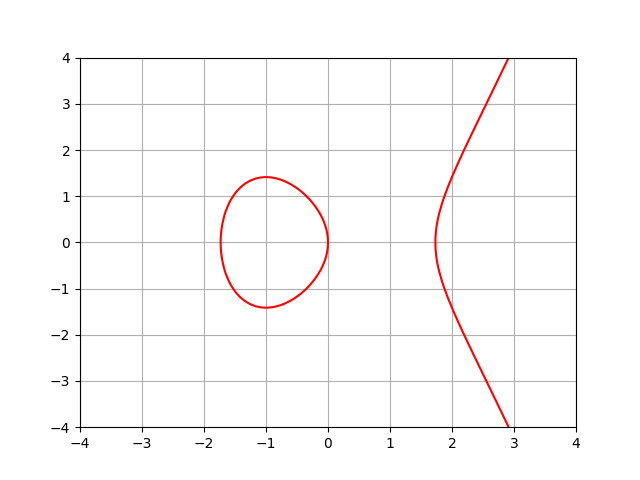
\includegraphics[width=\linewidth,keepaspectratio]{2.png}
    \end{minipage}
    \label{fig1}
    \caption{Eliptička krivulja $y^2 = x^3 - x + 5$ u projektivnoj/afinoj ravnini}
\end{figure}

\begin{nap}
    Treba napomenuti da svaka klasa ekvivalencije $(x, y, z)$ ima reprezentant $(x, y, 1)$ pa ćemo u nastavku koristiti koordinate točaka u ravnini unatoč tome što se nalazimo u projektivnom prostoru.
\end{nap}

\section{Eliptičke krivulje}

\begin{defin}
    Eliptička krivulja je glatka projektivna krivulja genusa 1 koja ima definiranu točku $\mathcal{O}$.
\end{defin}

Da bi razumijeli ovu definiciju potrebno je znanje algebarske geometrije. Kao što smo već ranije spomenuli, rad je pisan na način da poznavanje takvih karakterizacija nije potrebno. Općenito, eliptička krivulja $E(K)$ je nesingularna krivulja \footnote{nema "šiljaka" i ne presjeca se sama sa sobom} s barem jednom točkom čije točke zadovoljavaju jednadžbu
\begin{equation}
    \label{eq:1}
    F(x, y) = ax^3 + bx^2y + cxy^2 + dy^3 + ex^2 + fxy + gy^2 + hx + iy + j = 0
\end{equation}
gdje su $a, b, ..., j \in K$.

\begin{defin}
    Za točku $(x, y)$ na krivulji kažemo da je \textbf{signularna} ako vrijedi
    \[ \frac{\partial F}{\partial x} = \frac{\partial F}{\partial y} = 0 \]
\end{defin}

Nesingularnost eliptičke krivulje znači da nije singularna ni u jednoj točki, odnosno da komponente od $\nabla F$ u točkama koje zadovoljavaju jednadžbu ne iščezavaju istovremeno.

Jednadžba \ref{eq:1} ekvivalentna\footnote{dobije se transformacijom} je jednadžbi
\begin{equation}
    \label{eq:2}
    y^2 + a_1xy + a_3 y = x^3 + a_2 x^2 + a_4 x + a_6
\end{equation}
koju zovemo \textbf{generalizirana Weierstrassova forma}. To je forma koja vrijedi za sva polja i koristi se u kriptografij. Međutim, mi ćemo uz dodatne pretpostavke konstruirati kraću formu koja nam je pogodnija za račun. Pretpostavimo onda da je karakteristika polja različita od 2. Kako bi eliminirali $xy$ u jednadžbi \ref{eq:2} uvodimo supstituciju $y = y - \frac{a_1x + a_3}{2}$ te ju svodimo na:
\[ y^2 = x^3 + b_2x^2 + b_4x + b_6 \]
Nadalje, pretpostavimo da karakteristika polja nije 3 pa $x^2$ možemo eliminirati supstitucijom $x = x - \frac{b_2}{3}$ iz čega slijedi:
\[ y^2 = x^3 + c_4x + c_6 \]
odnosno
\begin{equation}
    \label{eq:3}
    y^2 = x^3 + ax + b
\end{equation}

Oblik \ref{eq:3} zovemo \textbf{kratka Weierstrassova forma}.

\begin{nap}
    Kada je karakteristika polja jednaka 2, dijeljenje s 2 nije moguće zato što je to množenje s inverzom od 2, a $1 + 1 = 0 = 2 \cdot 1 \ $ i $ \ 2\cdot x = 0, \forall x \in K$ pa 2 nema inverz.
    Analogno vrijedi i za karakteristiku 3.
\end{nap}
\begin{nap}
    Navedene supstitucije su izomorfizmi pa te transformacije smijemo raditi. Izomorfizam u kontekstu eliptičkih krivulja znači da krivulje, iako mjenjaju izgled, zadržavaju algebarska i geometrijska svojstva (npr. svojstva zbrajanja i rezultat se ne mjenjaju).
\end{nap}

U kratkoj Weierstrassovoj formi uvijet nesingularnosti možemo bolje definirati pomoću determinante polinoma s desne strane jednadžbe. Neka je
\begin{equation}
    \label{eq:cp}
    f(x) = x^3 + ax + b 
\end{equation}
\begin{theorem}
    \label{elipnult}
    Eliptička krivulja dana jednadžbom \ref{eq:3} je nesingularna ako i samo ako polinom \ref{eq:cp} nema višestrukih nultočki.
\end{theorem}
Dokaz ovog teorema zahtjeva algebarsku geometriju pa ga nećemo dokazivati. Iz teorema \ref{th:dt} znamo da je tvrdnja da polinom nema višestrukih nultočki ekvivalentna tvrdnji da je determinanta polinoma različita od $0$.
\begin{propozicija}
    \label{kubnadet}
    Neka je kubni polinom oblika $f(x) = x^3 + ax + b$, tada je njegova determinanta
    \[ D = -4a^3 - 27b^2 \]
\end{propozicija}
\begin{proof}
    Vodeći koeficijent od $f(x)$ je $1$, pa dokaz slijedi množenjem izraza \[(x - r_1)(x - r_2)(x - r_3)\] i izjednačavanjem/usporedbom s \[x^3 + ax + b\]
\end{proof}
\begin{korolar}
    Krivulja $y^2 = x^3 + ax + b$ je nesingularna ako i samo ako je
    \[ -4a^3 - 27b^2 \neq 0 \]
\end{korolar}
\begin{proof}
    Slijedi direktno iz \ref{elipnult} i \ref{kubnadet}
\end{proof}
\begin{nap}
    Diskriminanta je $0$ ako i samo ako $a = -3k^2$ i $b=2k^3$ za neki $k$.
\end{nap}
Sada možemo definirati eliptičku krivulju u nama pogodnoj formi.
\begin{defin}
    \label{elipkriv}
    Eliptička krivulja $E$ nad poljem $K$, karakteristike različite od 2 i 3, je skup točaka $(x, y) \in K \times K$ koje zadovoljavaju:
    \[ y^2 = x^3 + ax + b \]
    zajedno s točkom u beskonačnosti $\mathcal{O}$.
\end{defin}
\begin{nap}
    Eliptičku krivulju $E$ nad poljem $K$ označavat ćemo s $E(K)$.
\end{nap}
\begin{figure}[H]
    \begin{minipage}[c]{0.5\linewidth}
        \centering
        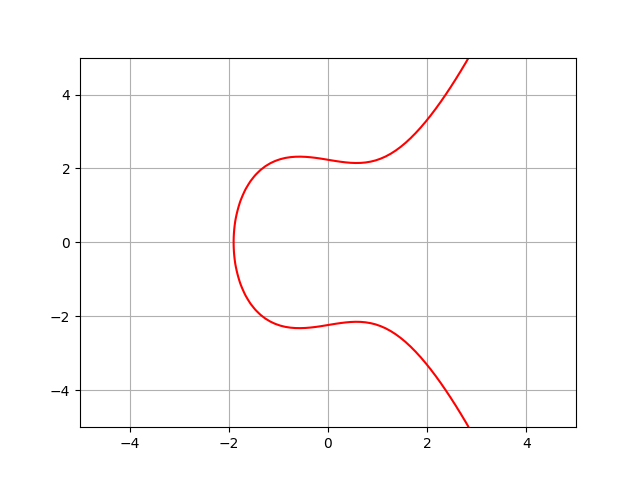
\includegraphics[width=\linewidth,keepaspectratio]{1.png}
        \caption{$E_1$: $y^2 = x^3 -x + 5$}
    \end{minipage}
    \begin{minipage}[c]{0.5\linewidth}
        \centering
        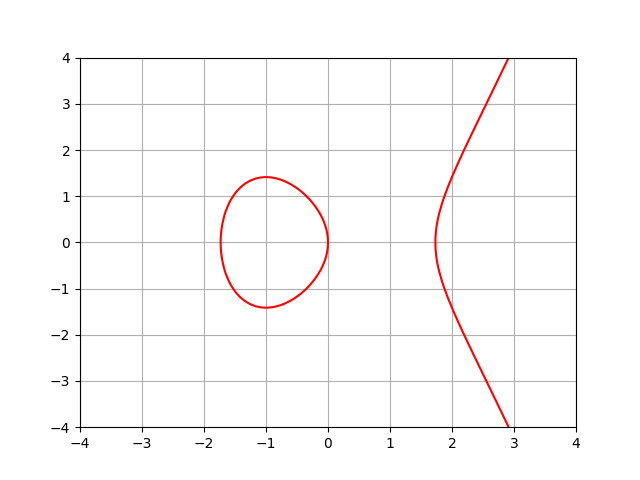
\includegraphics[width=\linewidth,keepaspectratio]{2.png}
        \caption{$E_2$: $y^2 = x^3 -3x$}
    \end{minipage}
\end{figure}

\begin{nap}
    U homogenim koordinatama jednadžba iz definicije \ref{elipkriv} postaje
    \[ zy^2 = x^3 + az^2x + bz^3 \]
    Presjek ove krivulje s pravcem u beskonačnosti nađemo tako da postavimo $z = 0$ što implicira $x^3 = 0$, odnosno u polju to znači $x = 0$. Sve točke oblika $(0, y, 0)$ zadovoljavaju jednadžbu, a taj skup je u projektivnoj geometrij točka $(0, 1, 0)$ koja je presjek krivulje s pravcem u beskonačnosti.
\end{nap}

\subsection{Operacije nad eliptičkim krivuljama}
U ovom poglavlju pretpostavljamo da je krivulja karakteristike različite od 2 i 3, odnosno koristimo definiciju \ref{elipkriv}. Također, svi geometrijski prikazi eliptičke krivulje su u $\mathbb{R}^2$. Najvažnije svojstvo eliptičkih krivulja jest da se na njima može uvesti operacija zbrajanja uz koju točke čine Abelovu grupu. To je moguće jer se zbog neprekidnosti krivulje može pokazati da točka u beskonačnosti $\mathcal{O}$ čini neutralni element za zbrajanje.

Svaku operaciju objasnit ćemo geometrijski te uvesti algebarsku definiciju na ravnini. Prva operacija koju ćemo uvesti je unarna operacija $-$. Kako je krivulja simetrična s obzirom na x os, za bilo koju točku $P$ možemo uzeti da $-P$ bude njena osnosimetrična točka.

\begin{figure}[H]
    \centering
    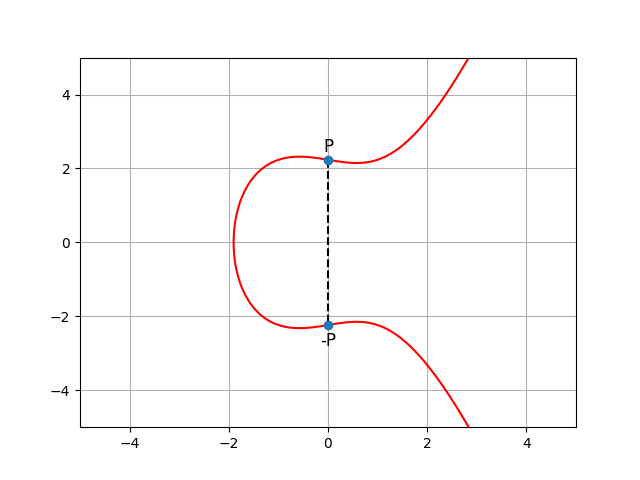
\includegraphics[width=0.6\linewidth,keepaspectratio]{4.png}
\end{figure}

\begin{defin}
    Neka je $E$ eliptička krivulja nad $K$ te $P = (x, y) \in E$. Unarna prefiksna operacija $-$ je funkcija $- : E \mapsto E$ sa sljedećim svojstvima:
    \begin{enumerate}
        \item Ako $P = \mathcal{O}$, onda $-P = \mathcal{O}$
        \item Ako $P \neq \mathcal{O}$, onda $-P = -(x, y) = (x, -y)$
    \end{enumerate}
\end{defin}
\begin{nap}
    $\mathcal{O}$ leži na $xz$ ravnini iz čega proizlazi prvo svojstvo prethodne definicije.
\end{nap}

Prije definiranja operacije zbrajanja, iskažimo teorem koji će nam biti motivacija za zbrajanje.

\begin{theorem}
    Eliptička krivulja sjeće pravac u točno 3 točke uzimajući u obzir njihove kratnosti.
\end{theorem}
\begin{proof}
    Dokaz uvrštavanjem jednadžbe pravca $y = mx + c$ u jednadžbu krivulje \ref{eq:cp} i raspisivanjem izraza u polinom trećeg stupnja tvrdnja slijedi iz fundamentalnog teorema algebre.
\end{proof}

Operaciju zbrajanja nad krivuljama uvest ćemo geometrijski. Uzmimo neke točke $P$ i $Q$ koje leže na krivulji. Povućemo li pravac kroz te dvije točke, krivulja sjeće jedinstvenu treću točku $R$. Znamo da treća točka sigurno postoji zbog točke u beskonačnosti $\mathcal{O}$. Za rezultat zbrajanja $P + Q$ uzet ćemo točku $-R$, odnosno osnosimetričnu točku točke $R$. 

U ovakvom zbrajanju imamo par specifičnih slučajeva. Prvi slučaj je pri zbrajanju s točkom $\mathcal{O}$. Tada je ta točka neutralni element i vrijedi $P + \mathcal{O} = P = \mathcal{O} + P$. 

Drugi slučaj je kad točku zbrajamo sa samom sobom, odnosno kada je $P = Q$. Tada za pravac koristimo tangentu krivulje u točki $P$. 

Treći slučaj je kad su točke okomite jedna na drugu, odnosno kada je $P = -Q$, tada $P + Q = P - P = \mathcal{O}$.

\begin{figure}[H]
    \begin{minipage}[c]{0.5\linewidth}
        \centering
        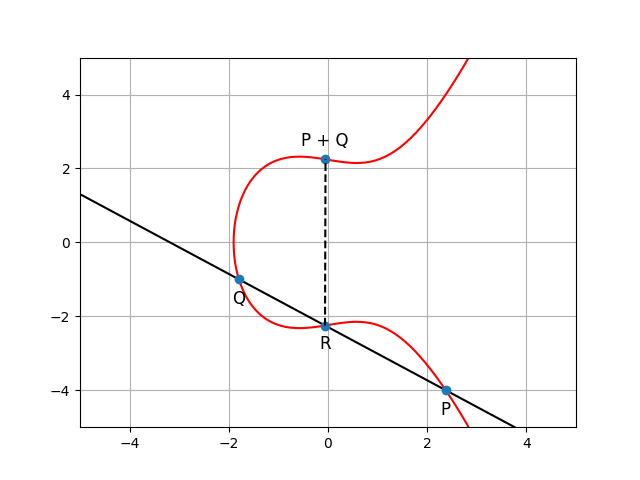
\includegraphics[width=\linewidth,keepaspectratio]{5.png}
    \end{minipage}
    \begin{minipage}[c]{0.5\linewidth}
        \centering
        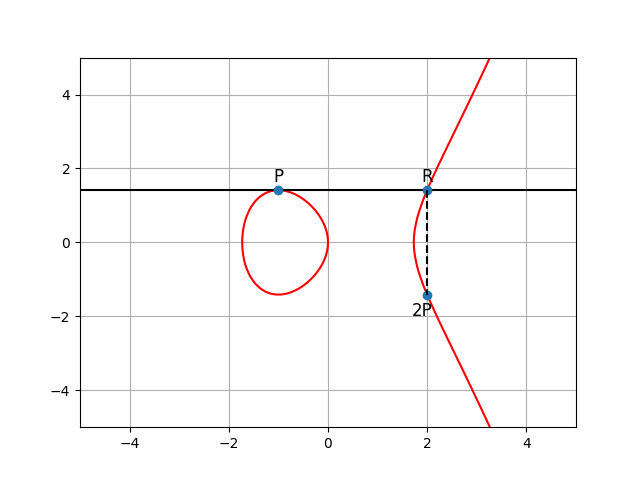
\includegraphics[width=\linewidth,keepaspectratio]{6.png}
    \end{minipage}
\end{figure}

\begin{nap}
    Treba napomenuti da postoji i slučaj kada je točka $P$ točka infleksije. Tada tangenta točke $P$ sjeće krivulju 3 puta u toj točki pa je u tom slučaju $P + P = P$.
\end{nap}

Definirajmo algoritam za zbrajanje točaka na krivulji.

\begin{defin}[Algoritam zbrajanja u $\mathbb{R}^2$]
    Neka je
    $E: y^2 = x^3 + ax + b$
    eliptička krivulja te $P$ i $Q$ točke na krivulji.
    \begin{enumerate}
        \item Ako $P = \mathcal{O}$, onda $P + Q = Q$
        \item Analogno za $Q$
        \item Inače $P = (x_p, y_p)$ i $Q = (x_q, y_q)$
        \item Ako $Q = (x_p, -y_p)$, onda $P + Q = \mathcal{O}$
        \item Inače neka je 
            \[ \lambda = \begin{cases}
                \frac{y_q - y_p}{x_q - x_p}, & \text{ako} P \neq Q \\
                \frac{3x_p^2+a}{2y_p}, & \text{inače}
            \end{cases} \]
            i
            \[ x_r = \lambda^2 - x_p - x_q \]
            \[ y_r = \lambda(x_p - x_r) - y_p \]
            Tada je $P + Q$ jednak $R = (x_r, y_r)$.
    \end{enumerate}
\end{defin}
\begin{proof}
    Prve 4 tvrdnje pokazali smo geometrijski.
    Ako je $P$ različit od $Q$, onda je $\lambda$ koeficijent smjera pravca kroz $P$ i $Q$. Ako je $P$ jednak $Q$, onda je $\lambda$ koeficijent smjera tangente kroz $P$. Iz toga slijedi da je pravac dan jednadžbom $y = \lambda (x - x_p) + y_p$. Neka je $\upsilon_p = y_p - \lambda x_p$.
    Uvrštavanjem jednadžbe pravca $y = \lambda x + \upsilon_p$ u jednadžbu krivulje imamo
    \[ (\lambda x + \upsilon_p)^2 = x^3 + ax + b \]
    odnosno
    \[ x^3 - \lambda^2x^2 + (a - 2\lambda\upsilon_p)x + (b - \upsilon_p^2) = 0 = (x - x_1)(x - x_2)(x - x_3) \]
    BSO neka su $x_1 = x_p$ i $x_2 = x_q$. Množenjem desne strane i promatranjem koeficijenta uz $x^2$ imamo $-\lambda^2 = - x_p - x_q - x_3$ iz čega slijedi jednadžba od $x_r$. $y_r$ je osnosimetrična točka nultočke $x_3$. Kako je ta točka $y = \lambda x_r + \upsilon_p$, slijedi $y_r = -y$. 
\end{proof}

Kao što je već spomenuto, od velike važnost u teoriji eliptičkih krivulja je da zbrajanje čini Abelovu grupu.
\begin{theorem}
    Neka je $E$ eliptička krivulja. Operacija zbrajanja na $E$ je Abelova grupa, odnosno vrijede slijedeća svojstva:
    \begin{enumerate}
        \item Asocijativnost: $\\
            \forall P, Q, R \in E, \enspace (P + Q) + R = P + (Q + R)
            $
        \item Postojanje neutralnog elementa: $\\
            \forall P \in E, \enspace P + \mathcal{O} = \mathcal{O} + P = \mathcal{O}
            $
        \item Postojanje inverznog elementa: $\\
            \forall P \in E, \enspace P + (-P) = \mathcal{O}
            $
        \item Komutativnost: $\\
            \forall P, Q \in E, \enspace P + Q = Q + P
            $
    \end{enumerate}
\end{theorem}
\begin{nap}
    Operacija zbrajanja je po definicij zatvorena. Zadnja 3 svojstva su definicijska što smo ranije pokazali geometrijski. Dokaz asocijativnosti koristi geometrijsku algebru (npr. \cite{ASOCPROOF}) pa teorem nećemo dokazivati.
\end{nap}

\section{Eliptičke krivulje nad konačnim poljima}
Kriptografija eliptičkim krivuljama koristi eliptičke krivulje definirane nad konačnim poljima.
\subsection{Konačna polja}
\begin{defin}[Konačno polje]
    Konačno polje je polje s konačnim brojem elemenata i označavat ćemo ga s $\mathbb{F}_q$, gdje je $q$ broj elemenata polja.
\end{defin}
\begin{primjer}
    Primjer takvog polja je skup cijelih brojeva modulo $p$ koji označavamo s $\mathbb{Z}/pZ$. Lako se pokaže da je takav skup s operacijama zbrajanja i množenja modulo $p$ polje.
\end{primjer}
\begin{defin}[Red polja]
    Za broj elemenata konačnog polja kažemo da je \textbf{red} konačnog polja.
\end{defin}
Polje reda 2 je degenerativno jer sadrži samo $0$ i $1$ pa ćemo uvijek uzimati da je $q > 2$.
\begin{nap}
    Konačno polje se još zove i Galoisovo polje (uz oznaku $GF(q)$).
\end{nap}
\begin{propozicija}
    Karakteristika konačnog polja mora biti prost broj.
\end{propozicija}
\begin{proof}
    Pretpostavimo suprotno, odnosno da je $n$ karakteristika koja nije prosta. To znači da $n$ možemo zapisati kao $n = a\cdot b$. Tvrdnja slijedi kontradikcijom zato što polje ne može imati dijeljitelje nule.
\end{proof}
\begin{lema}
    Ako je $p$ karakteristika polja $\mathbb{F}_q$, onda $\mathbb{F}_q$ sadržava $\mathbb{F}_p = \mathbb{Z}/p\mathbb{Z}$.
\end{lema}
\begin{proof}
    Neka je skup $S = \{0, 1, 1+1, 1+1+1, ..., (p-1) \cdot 1\}$ iz $\mathbb{F}_q$. Lako se pokaže da $S$ zadovoljava sva svojstva polja pa je $S$ potpolje od $\mathbb{F}_q$. Preostaje pokazati da je $S$ izomorfizam u $\mathbb{Z}/p\mathbb{Z}$. Izomorfizam je dan preslikavanjem $\phi: \mathbb{Z}/p\mathbb{Z} \mapsto S$ definiranim s $\phi(a) = 1 \cdot a$. Ovo je očito homomorfizam i po konstrukcij je surjekcija. Preslikavanje je injekcija jer ako $a \cdot 1 = b \cdot 1$, onda $(a - b) \cdot 1 = 0$ što implicira da $a \equiv b \enspace (mod \enspace p)$ zato što $p$ najmanji broj takav da $p \cdot 1 = 0$. $S$ je potpolje od $\mathbb{F}_q$ i izomorfizam u $\mathbb{Z}/p\mathbb{Z}$ što znači da $\mathbb{F}_q$ sadržava $\mathbb{F}_p$.
\end{proof}
$\mathbb{F}_q$ sadrži potpolje $\mathbb{F}_p$ pa je $\mathbb{F}_q$ vektorski prostor nad $\mathbb{F}_p$. Recimo da $\mathbb{F}_q$ ima dimenziju k i neka ima neku bazu $\{v_1, ..., v_k\}$. Svaki elementu $\mathbb{F}_q$ se može iskazat pomoću linearne kombinacije vektora baze gdje su koeficijenti elementi iz $\mathbb{F}_p$. Kako svaki koeficijent može biti jedan od p elemenata iz $\mathbb{F}_p$, slijedi da postoji $p^k$ linearnih kombinacija.
\begin{korolar}
    Konačno polje reda $q$ postoji onda i samo onda ako $q = p^k$ gdje je $p$ prost broj i $k \in \mathbb{Z}$.
\end{korolar}
\begin{nap}
    Uočimo da za svaku potenciju prostog broja $q = p^k$ postoji jedinstveno (do na izomorfizam) polje s $p$ elemenata.
\end{nap}

Iz prijašnjih tvrdnji slijedi da ukoliko $q = p^k$, onda postoji $\mathbb{F}_q$ čija je jedna od realizacija $\mathbb{Z}_p/f(x)$ gdje je $f(x)$ ireducibilni\footnote{nije djeljiv} polinom stupnja $k$ nad $\mathbb{Z}_p$. Elementi takvog polja su polinomi nad $\mathbb{Z}_p$ stupnja manjeg ili jednakog $k-1$.

\begin{nap}
    Zbrajanje i množenje vrše se uz proizvoljan $f(x)$ pa postoje pravila konstrukcije ireducibilnog polinoma uz koje operacije postaju puno efikasnije. 
\end{nap}

Uzmemo li $\mathbb{F}_{2^m}$ kao jedno takvo polje te $f(x)$ ireducibilni polinom stupnja $m$ nad $\mathbb{F}_2$, element tog polja možemo reprezentirati nizom od $m$ bitova. Iz toga je jasno zašto su nam polja oblika $\mathbb{F}_{2^m}$ značajna u primjeni.

Suma dva polinoma $A(x)$ i $B(x)$ iz $\mathbb{F}_{2^m}$ je
\[ C(x) = \sum_{i = 0}^{m - 1} (a_i + b_i) x^i \]
gdje se zbrajanje koeficijenata $a_i$ i $b_i$ vrši modulo 2. Kako je
\[ a_i + b_i \equiv a_i - b_i \ (mod\ 2) \]
slijedi da je operacija zbrajanja jednaka operacij oduzimanja.
\begin{nap}
    Primjetimo da je operacija zbrajanja modulo 2 ekvivalentna operacij XOR\footnote{ekskluzivno ili}($\oplus$) po komponentama te da ne ovisi o bazi.
\end{nap}

Za razliku od zbrajanja, baza utječe na rezultat množenja. Neka su opet $A(x)$ i $B(x)$ iz $\mathbb{F}_{2^m}$ te
\[ C(x) = A(x) \cdot B(x) = \prod_{i = 0}^{2m - 2} c_i x^i \]
gdje
\[
\begin{split}
    c_o & \equiv a_o b_o \ (mod \ 2) \\
    & \vdots \\
    c_{2m - 2} & \equiv a_{m-1} b_{m-1} \ (mod \ 2)
\end{split}
\]
Vidimo da će množenjem na ovakav način rezultat $C(x)$ biti stupnja većeg od $m-1$ pa operacija kao takva neće biti zatvorena u $\mathbb{F}_{2^m}$ zbog čega se množenje definira slično kao na prostim poljima. Operacija množenja vrši se modulo ireducibilan polinom $f(x)$.

\begin{primjer}
    Neka su $A(x) = x^3 + x + 1$ i $B(x) = x^2 + x$ polinomi iz $F_{2^4}$. Zbroj tih polinoma jednak je \[C(x) = (1+0\  mod\  2)x^3 + (0+1 \  mod\  2)x^2 + (1+1 \  mod\  2)x + (1+0 \  mod\  2) \] odnosno \[C(x) = x^3 + x^2 + 1\]
    Polinomi kao bitni nizovi veličine $4$ su $A = 1011$ i $B = 0110$. Operacijom XOR $\oplus$ na $A$ i $B$ dobili bi isti rezultat \[C = 1011 \oplus 0110 = 1101\] Za množenje ovakvih polinoma dodatno moramo odrediti ireducibilan polinom $f(x) \in \mathbb{F}_{2^4}$ stupnja $4$. Uzmimo za $f=1000$ odnosno $f(x)=x^3$. Umnožak $A(x)$ i $B(x)$ sada je;
    \[ \begin{split}
        C(x) & \equiv (x^3 + x + 1) \cdot (x^2 + x) \ (mod\  f(x)) \equiv \\
        & \equiv x^5 + x^4 + x^3 + (1+1\  mod\  2)x^2 + x \ (mod\  f(x)) \\
        & \equiv x^5 + x^4 + x^3 + x \  (mod\  f(x)) \equiv x
    \end{split}\]
    Binarnim množenjem uz iznimku da bitove "režemo" na veličinu $4$ dolazimo do istog rezultata:
    \[ 1011 \cdot 0110 = 0000 + 10110 + 101100 + 0000000 = 100|0010 = 0010 \]
\end{primjer}
\begin{nap}
    Primjetimo da je polje $\mathbb{F}_{2^m}$ karatkeristike 2 pa se jednadžba eliptičke krivulje $E$ nad tim poljem transformira u
    \[ y^2 + xy = x^3 + ax + b \]
\end{nap}

\subsection{Krivulje nad $\mathbb{F}_{p}$}

Za eliptičke krivulje nad $\mathbb{F}_p$ vrijedi isti algoritam za zbrajanje, ali se sada operacije zbrajanja i množenja vrše modulo $p$.

\begin{primjer}
    Neka je $E(\mathbb{F}_7)$ eliptička krivulja nad poljem $\mathbb{F}_7$. Točke ove krivulje tražimo rješavanjem jednadžbi
    \[ y^2 \equiv x^3 + 7x + 5 \  (mod\  7) \]
    gdje je $x\in\{0,...,6\}$.
    Uzmemo li na primjer $x = 1$ imamo $1 + 7 + 5 = 13$ pa za $x = 1$ nema odgovarajuće točke $y$ budući da $y^2$ nije kongruentno $13$ modulo $7$.
    Uzmemo li $x = 5$ imamo $125 + 35 + 5 = 165$, a kako je $5^2 \equiv 2^2 \equiv 165 \  (mod \ 7)$ za $x = 5$ slijedi da su $(5, 2)$ i $(5, 5)$ točke na eliptičkoj krivulji.
    Ponovimo li ovaj proces za preostalih $5$ $x$-eva pronalazimo da su točke ove krivulje 
    \[E(\mathbb{F}_7) =  \{ \mathcal{O}, (3, 2), (3, 5), (5, 2), (5, 5), (6, 2), (6, 5)\}\]
    pa je red ove krivulje $7$.
\end{primjer}

\begin{primjer}
    Neka je $E(\mathbb{F}_5) = \{ \mathcal{O}, (0, 1), (0, 4), (2, 1), (2, 4), (3, 1), (3, 4), (4,2), (4, 3) \}$ eliptička krivulja nad $\mathbb{F}_5$. 
    Izračunajmo $R = P + Q$ za $P = (3, 1)$ i $Q = (2, 4)$ algoritmom za zbrajanje.
    \[ \lambda \equiv \frac{4 - 1}{2 - 3} \equiv 2 \ (mod\  5)\]
    \[ x_r \equiv \lambda^2 - x_p - x_q \equiv 4 - 3 - 2 \equiv 4 \  (mod\  5)  \]
    \[ y_r \equiv \lambda(x_p - x_r) - y_p \equiv -2 - 1 \equiv 2 \  (mod\  5) \]
    \begin{figure}[H]
        \centering
        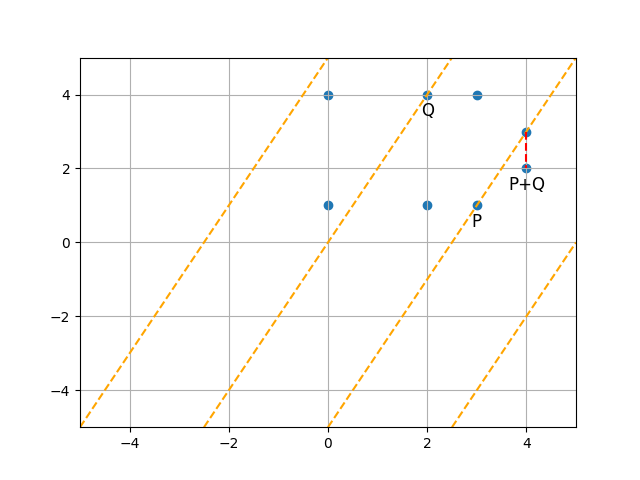
\includegraphics[width=0.8\linewidth,keepaspectratio]{7.png}
    \end{figure}
\end{primjer}

Kako bi napravili kvalitetan izbor krivulje za primjenu, potrebno je poznavanje veličine reda grupe $E(\mathbb{F}_p)$. Svakoj točki $x$ (ima ih $p$) mogu biti pridružene 2 točke $y$ pa znamo da je maksimalan broj točaka eliptičke krivulje nad poljem $p$ manji od $2p + 2$ ($2p$ točaka i točka u beskonačnosti). Precizniju među od navedene dat ćemo teoremom bez dokaza.
\begin{theorem}[Hasse]
    Neka $\mathbb{F}_p$ konačno polje s $p$ elemenata i $E(\mathbb{F}_p)$ eliptička krivulja nad $\mathbb{F}_p$. Tada je
    \[ p + 1 - 2 \sqrt{p} \leq |E(\mathbb{F_p})| \leq p + 1 + 2 \sqrt{p} \]
\end{theorem}
\begin{nap}
    Veličina $t = p + 1 - |E(\mathbb{F}_p)|$ naziva se Frobeniusov trag i prema Hasseovom teoremu vrijedi $t = 2 \sqrt{p}$.
\end{nap}

Pokazalo se da se za kriptosustave formirane nad eliptičkim krivuljama koje imaju Frobeniusov trag jednak 1, ili ako je karakteristika polja dijelitelj Frobeniusovog traga, mogu kreirati djelotvorni napadi. Problem odabira dobre krivulje je daleko izvan okvira ovog rada.

Postoje deterministički algoritmi za izračun reda krivulje od kojih ćemo neke spomenuti. Jedan takav algoritam je Lang-Trotterova metoda.

\begin{defin}[Legendreov simbol]
    Neka je konačno polje $F_p$ i $p$ neparan prost broj. Legendreov simbol je
    \[ \left(\frac{x}{\mathbb{F}_p}\right) = \begin{cases}
        1, & \enspace\text{ako}\enspace t^2 = x, \enspace \text{za neki} \enspace t \in \mathbb{F}_p \\
        -1, & \enspace\text{ako}\enspace t^2 = x \enspace \text{nema rješenje} \\
        0, & \enspace\text{ako je}\enspace x = 0
    \end{cases} \]
\end{defin}

\begin{theorem}
    Neka $E(\mathbb{F}_p)$ eliptička krivulja nad konačnim poljem u kratkoj Weierstrassovoj formi. Tada je
    \[ \#E(\mathbb{F}_p) = q + 1 + \sum_{x\in\mathbb{F}_p}^{} \left(\frac{x^3 + ax + b}{\mathbb{F}_p}\right) \]
\end{theorem}

Lang-Trotterov algoritam tvrdi da su tragovi na familiji eliptičkih krivulja "dobro" distribuirani. Vremenska kompleksnost algoritma je $O(pln^2p)$. Postoje algoritmi s boljim kompleksnostima kao što su Shanks-Maestrova metoda i Schoofov algoritam. Schoofov algoritam za dano polje $F_p$ računa točnu vrijednost Frobeniusovog traga u $O(ln^8p)$ bitovnih operacija. Algoritam\footnote{Schoof-Elkies-Atkin} je kasnije dodatno poboljšan na kompleknost $O(ln^6p)$. Schoofov algoritam radi na način da prvo odredimo skup malih prostih brojeva $l$ takvih da je njihov produkt veći od $4\sqrt{p}$ (po Hasseovom teoremu). Zatim za svaki element skupa $l$ računamo $t$ modulo $l$. Metoda završava korištenjem kineskog teorema o ostacima rekonstruirajući trag krivulje.

\chapter{Kriptografija javnog ključa}

\begin{defin}
    Kriptografija je znanost matematičkih tehnika vezanih uz zaštitu informacija.
\end{defin}

\section{Uvod}
Kriptografija javnog ključa revolucionizirala je sigurnost komunikacije eliminirajući potrebu za unparijednim dogovorom oko tajne. Kriptografija javnog ključa zasniva se na paru ključeva; javnom ključu za enkripciju (šifriranje) i privatnom ključu za dekripciju (dešifriranje). Cilj je pronaći što bolju jednosmjernu funkciju. U tu svrhu radimo eksperiment $\text{Invert}_{\mathcal{A}, f}(n)$;
\begin{enumerate}
    \item Odaberi $x\in\{0, 1\}^n$ uniformno i izračunaj $y = f(x)$
    \item $\mathcal{A}$ dobija $y'$ i vraća $x'$
    \item Ishod eksperimenta je $1$ ako $f(x') = y$, $0$ inače
\end{enumerate}
\begin{nap}
    Polinomijalno vrijeme izvođenja $\mathcal{A}$ može ovisiti o $n$, odnosno $\mathcal{A}$ dodatno prima $1^n$ što zovemo sigurnosni parametar.
\end{nap}

\begin{defin}
    Za funkciju $f: \{0, 1\}* \mapsto \{0, 1\}*$ kažemo da je jednosmjerna ako vrijedi slijedeće:
    \begin{enumerate}
        \item Postoji polinomijalan algoritam $M_f$ takav da $M_f(x) = f(x), \forall x$
        \item Za svaki vjerojatnostni polinomijalan algoritam $\mathcal{A}$, postoji zanemariva $\epsilon(n)$ takva da
    \end{enumerate}
    \[ P(\text{Invert}_{\mathcal{A}, f}(n) = 1) \leq \epsilon(n) \]
\end{defin} 

U kriptografij javnog ključa, ključevi su direktno povezani s jednosmjernim funkcijama. Uz poznavanje javnog ključa, funkcija je jednosmjerna, dok uz poznavanje privatnog ključa funkcija postaje dvosmjerna. Drugi naziv za kriptosustav javnog ključa je \textbf{asimetrični kriptosustav}.

\begin{defin}
Asimetrični kriptosustav definiramo kao uređenu petorku $(\mathcal{M}, \mathcal{C}, \text{Gen}, \text{Enc}, \text{Dec})$ gdje je:
\begin{enumerate}
    \item $\mathcal{M}$ prostor poruka.
    \item $\mathcal{C}$ prostor šifrata.
    \item $\text{Gen}$ stohastički generator ključeva ($(pk, sk) = \text{Gen}$).
    \item $\text{Enc}(m, pk)$ funkcija šifriranja ($c =\text{Enc}(m, pk)$).
    \item $\text{Dec}(c, sk)$ funkcija dešifriranja ($m = \text{Dec}(c, sk)$).
\end{enumerate}
\end{defin}

\begin{nap}
    Generator uobičajeno prima i sigurnosni parametar $1^n$.
\end{nap}

\begin{primjer}[RSA]
    Jedan primjer asimetričnog kriptosustava je RSA \footnote{Rivest-Shamir-Adleman} koji se zasniva na činjenici da je za pozitivne cijele brojeve $e,d,n$ takve da \[\forall m\in\mathbb{N}, m\leq n \  \text{i} \  (m^e)^d \equiv m \  (mod \ n)\] teško pronaći $d$ ako znamo $e$ i $n$. Neka je $n = pq$ gdje su $p$ i $q$ prosti brojevi te neka su $\mathcal{M} = \mathcal{C} = \mathbb{Z}_n$. Nadalje,
    \[ Gen = ((n, e), (n, d)) \]
    \[ Enc(m, (n, e)) =  m^e \  (mod \ n) \]
    \[ Dec(c, (n, d)) = c^d \  (mod \ n) \]
    gdje su ključevi takvi da vrijedi:
    \[n = pq\] 
    \[gcd(e,\lambda(n)) = 1\]
    \[d \cdot e \equiv 1 \  (mod\ \lambda(n))\]
    \[\lambda(n)=lcm(p-1, q-1)\]
    Za primjer uzmimo $p = 61$ i $q = 53$. Iz toga imamo da je $n = 3233$. Pomoću euklidovog algoritma računamo da je $\lambda(n) = 780$. Sada biramo $e$ relativno prost s $780$ pa neka je $e = 17$. $d$ izračunamo pomoću $e$ i $\lambda(n)$. Iz toga imamo da je šifrat $c = m^{17}\enspace mod \enspace 3233$ i poruka $m = c^{413} \enspace mod \enspace 3233$.
\end{primjer}

Kako bi se osigurala kvalitete kriptosustava uvedeni su sigurnosni modeli kojima se ispituju svojstva sustava. Mi ćemo opisati dva najznačajnija zahtjeva:

\begin{defin}[Zahtjev ispravnosti]
    Za asimetrični kriptosustav kažemo da je ispravan ako
    \[\forall m \in \mathcal{M} \  \text{i} \  \forall (pk, sk) \  \text{generiran pomoću} \  \text{Gen} \  \text{vrijedi}:
    \text{Dec}(\text{Enc}(m, pk), sk) = m \]
\end{defin}

\begin{theorem}[Fermatov mali teorem]
    \label{fermat}
    Neka je $p$ prost broj i $a$ cijeli broj. Vrijedi
    \[ a^p \equiv a \  (mod \  p) \]
\end{theorem}

\begin{primjer}
    Provest ćemo zahtjev ispravnosti na RSA. Trebamo pokazati da $(m^e)^d \equiv m \  (mod \  pq)$.
    Kako je $\lambda(n)$ dijeljiv s $p-1$ i $q-1$, za $k, h \in \mathbb{N}$ imamo $ed - 1 = h(p - 1) = k(q - 1)$.
    Sada ako $m \equiv 0 \  (mod \  p)$ onda $m^{ed} \equiv 0 \ (mod \  p)$. Inače $m^{ed} = m^{ed-1}m = m^{h(p-1)}m = (m^{p-1})^hm$
    pa po teoremu \ref{fermat} imamo $(m^{p-1})^hm \equiv m \ (mod \ p)$
    Analogno napravimo i za $m^{ed} \equiv 0 \ (mod \  q)$.
    Iz toga slijedi $(m^e)^d \equiv m \ (mod \ pq)$.
\end{primjer}

Očito je da sustavi u kojima ne vrijedi zakon ispravnosti nisu od koristi. Od zahtjeva sigurnosti najznačajnij je IND-CPA (indistinguishability under chosen-plaintext attack). IND-CPA definira se igrom izazivača i protivnika.
Slijed igre je slijedeći:
\begin{enumerate}
    \item Izazivač generira par ključeva $sk$ i $pk$ te šalje ključ $pk$ protivniku
    \item Protivnik radi proizvoljan polinomijalan broj operacija i nakon toga šalje dva plaintexta $M_0$ i $M_1$ izazivaču
    \item Izazivač bira nasumičan bit $b\in\{0, 1\}$ i šalje "izazov" $C = Enc(M_b, pk)$ protivniku.
    \item Protivnik radi proizvoljan polinomijalan broj operacija i pogađa bit $b'$ 
\end{enumerate}
Kriptosustav je siguran ako protivnik ima zanemarivo malu prednost nad slučajnim pogađanjem, odnosno;

\begin{defin}[Zahtjev sigurnosti]
    Za asimetrični kriptosustav kažemo da je IND-CPA siguran ako
    \[\forall \mathcal{A}, \enspace \exists \epsilon(n) \enspace \text{t.d.} \enspace P(b = b') \leq \frac{1}{2} + \epsilon(n) \]
    gdje je $\mathcal{A}$ polinomijalni algoritam napadača, $\epsilon(n)$ zanemariva funkcija te $P$ vjerojatnost pobjede protivnika.
\end{defin}

\begin{nap}
    Ovu definiciju možemo interpretirati na način da se u sigurnim sustavima ne može dobiti nikakva informacija promatranjem šifrata.
\end{nap}

\section{Problem diskretnog logaritma}
Ne postoji formalan dokaz postojanja jednosmjernih funkcija pa njihovu egzistenciju moramo pretpostavit. Prilikom konstrukcije asimetričnih kriptosustava, odnosno jednosmjernih funkcija, najčešće se uzimaju u obzir teški matematički problemi iz teorije brojeva. Jedan takav problem zove se problem diskretnog logaritma.

\begin{defin}
    \label{DLP}
    Neka je $(G, *)$ konačna grupa, $g\in G$ i $H = \{g^i: i \geq 0\}$ podgrupa od $G$. Neka je $x \in \mathbb{Z}$ najmanji broj (zbog jedinstvenosti) takav da
    \[ h = g^x = \underbrace{g + \cdots + g}_{\text{x puta}} \]
    Ako takav $x$ postoji zovemo ga diskretni logaritam i označavamo s $log_g h$.
\end{defin}

Može li se generalni diskretni logaritam izračunati u polinomijalnom vremenu neriješen je problem u računalnoj znanosti. To znači da nije otkriven (ne kvantni) algoritam za izračun diskretnog logaritma zbog čega je potenciranje nad konačnim poljem dobar kandidat za jednosmjernu funkcije.

\begin{defin}[Red točke]
    Neka je $G$ grupa s neutralnim elementom $1$ i neka je $P\in G$. Za broj $n$ točke $P$ kažemo da je red točke ako je to najmanji broj takav da $P^n = 1$.
\end{defin}

\begin{propozicija}
    \label{reddjeljiv}
    Neka je $G$ konačna grupa. Svaki element od $G$ ima konačan red. Ako $a \in G$ reda $d$ i $k$ najmanji takav da vrijedi $a^k = e$, onda $d | k$.
\end{propozicija}

\begin{primjer}
    Neka je $G$ multiplikativna grupa od $E(\mathbb{F}_p)$ gdje za $P, Q\in E(\mathbb{F}_p)$ problem diskretnog algoritma predstavlja određivanje $d\in [0, n-1]$, pri čemu je $n$ red točke $P$, takav da $Q = nP$.
\end{primjer}

\subsection{Problem diskretnog logaritma za eliptičke krivulje}
\begin{defin}[ECDLP]
    Neka je $E$ eliptička krivulja nad $\mathbb{F}_p$ i neka su $Q$ i $P$ točke u $E(\mathbb{F}_p)$. Problem diskretnog logaritma za eliptičke krivulje je problem pronalaska $n \in \mathbb{N}$ takvog da je $Q = nP = \underbrace{P + \cdots + P}_{n}$.
    \[ n = \log_p(Q) \]
\end{defin}

\begin{nap}
    $n$ zovemo eliptički diskretni logaritam od $Q$ u odnosu na $P$.
\end{nap}

Kada su $E$ i $P$ ispravno odabrani, rješavanje diskretnog logaritma smatra se nemogućim uz pretpostavku da je red točke P dovoljno velik da je teško provjeriti sve mogućnosti za $d$.

Šifriranje u sustavima baziranim na problemu diskretnog logaritma za eliptičke krivulje obavlja se računanjem $nP$. Kao što smo već napomenuli, želimo da nam je funkcija šifriranja što efikasnija. Prvo primjetimo budući da je $E(\mathbb{F}_p)$ konačan, postoje cijeli brojevi $k > j$ takvi da je $kP = jP$. Tada je po propozicij \ref{reddjeljiv} ($k - j$) red točke $P$ što znači da je vrijednost $log_P(Q)$ element iz $\mathbb{Z}/(k-j)\mathbb{Z}$. Ukoliko znamo da je $n = n_o + i(k-j)$ jednostavno možemo staviti $log_P(Q) = n_oP$. Važnija stvar za primjetiti je da broj $n$ možemo zapisati u binarnom obliku $n = n_0 + n_1 2 + n_2 2^2 + ... + n_r 2^r$. Tada uz oznaku $P_i = 2^i P$, odnosno $P_i = 2 P_{i-1}$ imamo da je $nP = n_0 P_0 + n_1 P_1 + ... + n_r P_r$. Ukupno vrijeme izračuna na ovaj način je najviše $2r$, odnosno množenje smo sveli na logaritamsku kompleksnost $log_2(n)$, što nam omogućava računanje $nP$ za velike vrijednosti $n$.

Svi sustavi koji u definicij koriste grupu $\mathbb{Z}_p^*$ mogu se modificirati tako da koriste $E(\mathbb{Z}_p)$. Razlika je što budući da je eliptička krivulja aditivna umjesto potenciranja imamo uzastopno zbrajanje.

\begin{nap}
    ECDLP puno je teži problem nego diskretni logaritam multiplikativne grupe konačnog polja pa se ista sigurnost postiže za puno manju veličinu ključa.
\end{nap}

U nastavku navest ćemo neke od sustava zasnovane na ECDLP.

\section{ElGamalov kriptosustav}
Originalno, kriptosustav je koristio multiplikativnu grupu $G = (\mathbb{Z}/p\mathbb{Z})*$. Najbrži poznati algoritam za traženje diskretnog logaritma u $(\mathbb{Z}/p\mathbb{Z})*$ je kompleksnosti $e^{O((\log p)^{\frac{1}{3}} (\log\log p)^{\frac{2}{3}})}$ što znači da je po kompleksnosti ekvivalentan problemu faktorizacije. Modificiranjem problema da koristi grupu $E(\mathbb{F}_p)$ imamo slijedeći sustav:
\begin{defin}
    \textbf{ElGalmanov kriptosustav ECC} eliptičke krivulje $E(\mathbb{F}_p)$ nad konačnim poljem $\mathbb{F}_p$ i točkom $P\in E(\mathbb{F}_p)$ je uređena petorka $(\mathcal{M}, \mathcal{C}, \text{Gen}, \text{Enc}, \text{Dec})$ takva da:
    \begin{align*}
        \mathcal{M} & = E(\mathbb{F}_p) \\
        \mathcal{C} & = E(\mathbb{F}_p)^2 \\
        Gen = (pk, sk) & = (aP, a) \\
        Enc(m, pk) & = (kP, m + k \ pk) \\
        Dec((c_1, c_2), sk) & = c_2 - sk \ c_1
    \end{align*}
    gdje su $a, k \in \{ 1, 2, ..., n-1 \}$ nasumično generirani i $n$ red točke $P$.
\end{defin}

\begin{nap}
    Lako se vidi da je sustav ispravan. $\text{Dec}(c, sk) = c_2 - a \ c_1 = m + k(aP) - a(kP) = m + k(aP) - k(aP) = m$
\end{nap}

Uz doslovno prevođenje sustava $(\mathbb{Z}/p\mathbb{Z})^*$ na $E(\mathbb{F}_p)$ moramo uzeti u obzir i probleme koji se pojavljuju. Primjerice, moramo osmisliti algoritam koji će preslikati naše poruke u skup $\mathcal{M}$, odnosno točke na krivulji. Za to ne postoji deterministički algoritam pa se u ovom slučaju koristi probabilistički algoritam. Primjer jednog takvog algoritma temelji se na činjenici da polovinu svih elemenata čine kvadrati. Neka se otvoreni tekst sastoji od cijelih brojeva između $0$ i $M$. Za cijeli broj $m$ u $k$ koraka tražimo $x = mk + j$ gdje je $j\in\{1, 2, ..., k\}$ minimalan takav da $x^3 + ax + b$ bude kvadrat modulo $p$. Pokazuje se da je približna vrijednost da u $k$ koraka pronađemo takav $x$ dana s $1 - (\frac{1}{2})^k$ pa za npr. $k = 50$ imamo skoro gotovo siguran pogodak. Formulom $m = \lfloor \frac{x-1}{k} \rfloor$ vraćamo točku u otvoreni tekst.

TODO PRIMJER

\begin{nap}
    Ovim algoritmom poruka se znatno poveća što je također problematično.
\end{nap}


\section{Menezes-Vanstoneov kriptosustav}
Ovaj kriptosustav je varijanta ElGamalovog kriptosustava. Eliptičke krivulje koriste se za maskiranje, a otvoreni tekstovi i šifrati su uređeni parovi polja koji ne moraju biti točke eliptičke krivulje.

\begin{defin}
    \textbf{Menezes-Vanstoneov kriptosustav ECC} eliptičke krivulje $E(\mathbb{F}_p)$ nad konačnim poljem $\mathbb{F}_p$ i točkom $P\in E(\mathbb{F}_p)$ je uređena petorka $(\mathcal{M}, \mathcal{C}, \text{Gen}, \text{Enc}, \text{Dec})$ takva da:
    \begin{align*}
        \mathcal{M} & = (\mathbb{F}_p)^2 \\
        \mathcal{C} & = E(\mathbb{F}_p)^2 \\
        Gen = (pk, sk) & = (aP, a) \\
        Enc(m, pk) & = (kP, (m_1 Q_x, m_2 Q_y)) \\
        Dec((c_1, c_2), sk) & = (c_{2_1}/Q_x, c_{2_2}/Q_y)
    \end{align*}
    gdje su $a, k \in \{ 1, 2, ..., n-1 \}$ nasumično generirani za $n$ red točke $P$, $Q = sk c_1 = a c_1 = a(kP)$ i $c_{2_1}$, $c_{2_2}$ komponente $c_2$.
\end{defin}
U usporedbi s ElGamalovim kriptosustavom, ovaj sustav ima šifru od dvije točke umjesto četiri.

\section{Diffie-Hellman razmjena ključeva}
Kriptosustave koje smo do sada naveli su jednosmjeran način komunikacije u kojem jedna osoba ima privatni ključ, a druga javni. Kako bi mogli imati dvosmjernu sigurnu komunikaciju mora postojati protokol razmjene ključeva. Diffie-Hellman je najpoznatij i najranij praktični primjer javne razmjene ključeva. U kontekstu ovog rada nas specifično zanima eliptički Diffie-Hellman. Pretpostavimo da Alice želi uspostaviti tajni ključ s Bobom, ali je kanal njihove komunikacije javan. Najprije Alice i Bob dogovore se oko parametara $(p, a, b, P, n, h)$ gdje je $p$ prost red polja, $a$ i $b$ parametri krivulje, $P$ bazična točka reda $n$ i kofaktor $h$ koji ćemo mi ignorirati. Također, i Bob i Alice moraju imati svoj privatni ključ $d$ nasumično odabran iz $[1, n-1]$ i javni ključ $Q = dP$. Neka je Alice ključ $(d_A, Q_A)$ i Bobov ključ $(d_B, Q_B)$. Alice računa $(x_k, y_k) = d_A \cdot Q_B$ te Bob računa $(x_k, y_k) = d_B \cdot Q_A$. Sada je $x_k$ njihova zajednička tajna jer vrijedi: \[ d_A \cdot Q_B = d_A \cdot d_B \cdot P =  d_B \cdot d_A \cdot P = d_B \cdot Q_A \] Nakon uspostave zajedničkog tajnog ključa, Alice i Bob mogu komunicirati putem nekog od ranije navedenih kriptosustava.

\begin{primjer}
    (Primjer iz \cite{ECL})
    Alice i Bob žele imati siguran kanal komunikacije te su odabrali koristiti Menezes-Vanstoneov kriptosustav. Za eliptičku krivulju odabrali su $y^2 = x^3 + x + 1$ nad poljem $\mathbb{Z}_{31}$ te bazičnu točku $P = (9, 10)$. Iz toga slijedi da je $\#\mathbb{Z}_{31} = 34$ i točka $P$ reda $34$. Točke ove eliptičke krivulje prikazane su tablicom:
    \begin{table}[h]
        \centering
        \begin{tabular}{|c|c|c|c|c|c|c|c|c|c|c|c|}
        \hline
        $k$ & $k \times P$ & $k$ & $k \times P$ & $k$ & $k \times P$ & $k$ & $k \times P$ & $k$ & $k \times P$ & $k$ & $k \times P$ \\
        \hline
        1 & (9,10) & 7 & (6,24) & 13 & (27,10) & 19 & (5,22) & 25 & (16,23) & 31 & (23, 13) \\
        2 & (18,29) & 8 & (24,29) & 14 & (26,21) & 20 & (26,10) & 26 & (24,2) & 32 & (18, 2) \\
        3 & (23,19) & 9 & (16,8) & 15 & (5,9) & 21 & (27,21) & 27 & (6,7) & 33 & (9, 21)\\
        4 & (4,22) & 10 & (20,2) & 16 & (19,3) & 22 & (28,18) & 28 & (17,13) & 34 & $\mathcal{O}$ \\
        5 & (25,16) & 11 & (22,22) & 17 & (10,0) & 23 & (22,9) & 29 & (25,15) & & \\
        6 & (17,18) & 12 & (28,13) & 18 & (19,28) & 24 & (20,29) & 30 & (4,9) & & \\ 
        \hline
        \end{tabular}
    \end{table}
    Poistovjetimo $a = 1$, $b = 2$, ..., $z = 26$. Sada komunikaciju provode na slijedeći način:
    \begin{enumerate}
        \item Alice odabire tajni ključ $7$ i računa $7 \times P = (6, 24)$
        \item Bob odabire tajni ključ $12$ i računa $12 \times P = (28, 13)$
        \item Alice želi poslati poruku 'ok', odnosno $(15, 11)$. Odabire slučajan $k = 5$ te šifrira poruku slijedećim procesom; $(c_1, c_2) = 5 \times (28, 13) = (24, 29)$, $5 \times P = (25, 16)$ te $c_1 x_1 = 24\cdot 15 \ mod \ 31 = 19$ i $c_2 x_2 = 29\cdot 11 \mod \ 31 = 9$. Nakon toga šalje poruku $((25, 16), 19, 9)$.
        \item Nakon što primi poruku, Bob računa $(c_1, c_2) = 22 \times (25, 16) = (24, 29)$ zatim invertira elemente 24 i 29 modulo 31 koristeći Euklidov algoritam. Bob sada može očitati originalnu poruku: $(19\cdot 22, 9 \cdot 15) \ mod \ 31 = (15, 11)$, tj. 'ok'.
    \end{enumerate}
\end{primjer}

\chapter{Dodatno}
\section{Napadi na diskretni logaritam eliptičke krivulje}
Jedna od strategija napada na problem diskretnog logaritma je svođenje problema na jednostavnij problem diskretnog logaritma. To se radi algoritmima koji reduciraju problem diskretnog logaritma za eliptičke krivulje na problem diskretnog logaritma za multiplikativne grupe nad konačnim poljem.
Jedan takav napad zove se MOV napad. Radi po principu Weilovog uparivanja koji uzme dvije točke s krivulje i preslika ih u točku konačnog polja. Supersingularne eliptičke krivulje, odnosno eliptičke krivulje za koje vrijedi $a \equiv 0 \ (mod \ p)$ posebno su osjetljive na ovaj napad. Postoji i napad imenom Frey-Ruck koji radi vrlo slično, ali umjesto Weilovog uparivanja koristi Tate-Lichtenbaum uparivanje. Uz to postoje i razni napadi nad općenitim eliptičkim krivuljama kao npr. Baby step/Giant step i Pollardove metode. Puno više o tome možete proučiti u \cite{ECRYPT}.

\section{Poboljšanje efikasnosti eliptičkih krivulja}
Prostornu efikasnost možemo poboljšati drugačijom reprezentacijom točaka. Znamo da su eliptičke krivulje simetrične s obzirom na $x$ os. Broj bitova za reprezentaciju točke na eliptičkoj krivulji možemo za duplo smanjiti primjetimo li da uvijek postoje dvije točke za neki $x$ čija je razlika u $y$ samo predznak. To znači da bilo koju točku $P = (x, y)$ možemo prikazati pomoću $x$ koordinate i bita $b$.

Računsku efikasnost možemo poboljšati homogenim koordinatama eliminirajući potrebu za računanjem inverza modulo. U projektivnim koordinatama algoritam za zbrajanje je oblika
\[ R = \left(\lambda^2 - \frac{x_p}{z_p} - \frac{x_q}{z_q}, \lambda(\frac{x_p}{z_p} - \lambda^2 + \frac{x_p}{z_p} + \frac{x_q}{z_q}) - \frac{y_p}{z_p}, 1\right) \]
gdje se sve operacije vrše modulo $p$. Kako su homogene koordinate točke klasa ekvivalencije smijemo ih množiti s
\[ z_p z_q (x_q z_p - x_p z_q)^3 \neq 0 \ mod \ p \]
pa imamo da je $R$ oblika
\[ R = (vw, u(v^2x_pz_q - w) - v^3y_pz_q, z_pz_qv^3) \]
gdje izrazi $u$,$v$ i $w$ ne sadrže inverze.

\begin{thebibliography}{30}
\addcontentsline{toc}{chapter}{Literatura}


\bibitem{EC1}
{\sc Henry McKean , Victor Moll}, {\em Elliptic curves}

\bibitem{CRYPT1}
{\sc Menezes A. J. , van Oorschot P. C., Vanstone S. A.}, {\em Handbook of applied cryptography}

\bibitem{CRYPT2}
{\sc Katz J., Lindell Y.}, {\em Introduction to modern cryptography}

\bibitem{ECRYPT}
{\sc Kenneth H. Rosen}, {\em Eliptic curves, Number theory and cryptography, Second edition}

\bibitem{EC2}
{\sc Kokanović A.}, {\em Eliptičke krivulje u kriptografiji}, Sveučilište J.J.Strossmayera u Osijeku, Odjel za matematiku

\bibitem{EC3}
{\sc Musulin Z.}, {\em Eliptičke krivulje i kriptiranje}, Sveučilište u Zagrebu, PMF

\bibitem{ASOCPROOF}
https://building-babylon.net/2024/05/26/associativity-of-the-group-law-on-a-non-singular-elliptic-curve-via-the-cayley-bacharach-theorem/

\bibitem{ECL}
{\sc Dino Sejdinović}, {\em Eliptičke krivulje u kriptografiji}, Osječki matematički list 6, 85-97

\bibitem{KONP}
https://web.math.pmf.unizg.hr/~duje/ecc/konpolja.html

\end{thebibliography}

\end{document}
